\section{Introduction}
This chapter will outline the usage of Br\'eguet's range equations in two methods for finding the Pareto frontier of optimal range and loiter time tradeoffs for an aircraft, given specific performance characteristics. Additionally, a method for determining a Pareto frontier will be established for the range of an aircraft's flight and its respective loiter time and will be referred to as an aircraft's tradeoff frontier. Lastly, the application of this approach will be explained in detail.\par
\section{Current Methodology}
The current methodology is derived from the service rules determined by the National Air Intelligence Agency. The defining rules that govern the flight path for combat air patrol control the inputs and outputs of the flight plan generated by NASIC. The steps include warmup (1), climb to cruise altitude (2), cruise and drop external fuel tanks (3), descend to loiter altitude and loiter at the profile for maximum endurance (4), descend to 10,000 feet (5), accomplish two minutes of combat (6), drop external tanks (7), climb to cruise altitude (8), cruise back to initial point (9), land with reserve fuel generally at 20 minutes plus 5\% initial fuel load (10) and are shown in Figure \ref{fig: serviceRules}.\par
\begin{figure}[H]
    \centering
    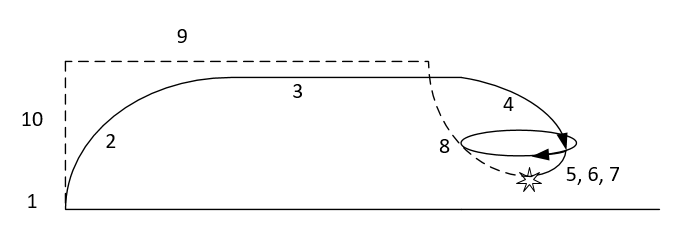
\includegraphics{Thesis/Method/CombatServiceRules.PNG}
    \caption{Visualization of Combat Air Patrol Service Rules}
    \label{fig: serviceRules}
\end{figure}
The options for a flight developed by NASIC and defined by combat air patrol service rules require either a distance to a interest location or a distance to the interest location and a wanted loiter time at the location. NASIC then develops the tradeoffs for loiter altitude, loiter time, or other flight options. The change in loiter altitude can effect the ability of an aircraft to loiter given a range. NASIC calculates an approximate tradeoff profile of loiter time given range between altitudes by linearly interpolating the loiter time between altitudes of 5,000 feet. The method is tedious and labor and time intensive for different flight profiles and calculations for loiter time between altitudes.
\section{Deriving Br\'eguet Equations}
\label{section: derive equations}
Two main equations are derived from the general range equation seen in Eq. \ref{eqRangeEq}, Eq. \ref{eq:genRangeFull} and Eq. \ref{eq: NLRange}. Eq. \ref{eq:genRangeFull} is used when assuming a linear fuel loss for an aircraft and Eq. \ref{eq: NLRange} is used when assuming a logarithmic fuel loss for an aircraft. The first logically flows from the need to maximize range while assuming a constant thrust specific fuel consumption (constant altitude and throttle setting). Maximizing $V/T_A$ will maximize range and $T \approx T_R = D$ where $D$ is drag. Thus, to maximize range, the aircraft must be flown at $(D/V)_{min}$. The following equivalent equations follow from the assumption that the aircraft will fly at straight, level, unaccelerated flight.
\begin{align}
    T_A&=D = C_Dq_{\infty}S \dfrac{W}{L} = \dfrac{C_Dq_{\infty}S(W)}{C_Lq_{\infty}S} = \dfrac{C_D}{C_L}W\\
    L &= W = C_Lq_{\infty}S = C_L\dfrac{1}{2}\rho_{\infty}V^2_{\infty}S \Rightarrow V_{\infty} = \sqrt{\dfrac{2W}{\rho_{\infty}C_LS}}
    \label{eq: VequivalentEq}
\end{align}
These equations can be used in the general range equation shown in Eq. \ref{eq:genRangeFull}.
\begin{equation}
\label{eq:genRangeFull}
    \begin{aligned}
        R &= \int_{W_f}^{W_i}\sqrt{\dfrac{2W}{\rho_{\infty}C_LS}}\left(\dfrac{1}{TSFC}\right)\left(\dfrac{C_L}{C_D}\right)\left(\dfrac{1}{W}\right)dW\\
        R &= \int_{W_f}^{W_i}\sqrt{\dfrac{2W}{\rho_{\infty}S}}\left(\dfrac{1}{TSFC}\right)\left(\dfrac{C_L^{1/2}}{C_D}\right)\left(\dfrac{1}{W}\right)dW\\
    \end{aligned}
\end{equation}
Further simplifying assumptions are used in general aircraft performance in \cite{IntroACMechanics} to derive the following Bre\'guet range equation in Eq. \ref{eq:LinRangeEq}. These include a constant altitude which implies a constant density, $\rho_{\infty}$, a constant angle of attack which makes $C_L$ and $C_D$ constant, and similar to the general equation, TSFC is constant.
\begin{equation}
\label{eq:LinRangeEq}
    \begin{aligned}
        R &= \sqrt{\dfrac{2}{\rho_{\infty}S}}\left(\dfrac{1}{TSFC}\right)\left(\dfrac{C_L^{1/2}}{C_D}\right)\int_{W_f}^{W_i}\dfrac{dW}{\sqrt{W}}\\
        R &= \sqrt{\dfrac{2}{\rho_{\infty}S}}\left(\dfrac{2}{TSFC}\right)\left(\dfrac{C_L^{1/2}}{C_D}\right)(\sqrt{W_i}-\sqrt{W_f})
    \end{aligned}
\end{equation} \par
In addition to the linear range equation, another simplification of the general range equation involves assuming constant cruise velocity, a constant angle of attack, and a constant thrust specific fuel consumption. This equation is referred to in \cite{IntroACMechanics} as the constant speed cruise range equation. Using the general range equation in \ref{eq:genRangeFull} and substituting $V$ in for the equivalent formula presented in \ref{eq: VequivalentEq}, the following equation is derived.
\begin{equation}
    R = \dfrac{V}{TSFC}\left(\dfrac{C_L}{C_D}\right)\ln{\dfrac{W_i}{W_f}}
    \label{eq: NLRange}
\end{equation}
This equation is maximized when $V\dfrac{C_L}{C_D}$ is maximized or equivalently when $\dfrac{C_L^{1/2}}{C_D}$ is maximized.

\section{Range Determination}
Parameters for the flight plan can either be user-defined or be defined to maximize performance for a best case scenario. In the interest of simplicity, the T-37 will be used as a general example for how parameters are extracted for maximizing range performance and the F-15C will be used to identify parameters from the existing NASIC model. \par
The theoretical drag polar for an aircraft is shown in Eq. \ref{eq: dragpolar}.
\begin{equation}
    C_D = C_{D_0} + kC_L^2
    \label{eq: dragpolar}
\end{equation}
where $C_{D_0}$ is the parasitic drag coefficient and $k = 1/\pi A_Re$ where $A_R$ is the aspect ratio of the aircraft and $e$ is the Oswald's efficiency factor. Yechout \cite{IntroACMechanics} introduces the T-37's drag polar equation for an example that maximizes the $C_L/C_D$ and $C_L^{1/2}/C_D$. The drag polar equation for the T-37 is shown to be  
\begin{equation*}
    C_D = 0.02 + 0.057C_L^2.
\end{equation*}
In order to maximize $C_L/C_D$ and $C_L^{1/2}/C_D$, Eq. \ref{eq:maxlift} is used to solve for $C_L$ where
\begin{equation*}
    C_{L_{MR}} = \sqrt{\dfrac{0.02}{3(0.057)}} = 0.342.
\end{equation*}
Using this value for $C_L$, $C_D$ can be calculated using the T-37 drag polar.
\begin{equation*}
    C_D = 0.02 + 0.057(0.342)^2 = 0.0267
\end{equation*}
As a result, flying at these values for maximizing $C_L$ and $C_D$ will maximize range and endurance \cite{IntrotoAero}. These values will allow for the use of a continuous range equation introduced in Eqs. \ref{eq:LinRangeEq} and \ref{eq: NLRange}. \par
\subsection*{Linear Range Determination}
Beginning with the formulation for the linear range equation, the intercept for maximum range and the intercept for starting fuel must be determined. Since the flight pattern will include an initial warm-up, take-off, and climb, the developed method assumes that the fuel burn and distance from initial starting point are given, though these can also be calculated using optimal climbing conditions discussed by Yechout \cite{IntroACMechanics}. To identify the point where the aircraft starts its egress to a point of interest, this model requires the vertical value to be in terms of fuel reserve. Thus, to determine the slope of this line, the fuel burn must be converted to the fuel reserve of the aircraft. For example, assume the T-37 flies 1.5 miles on its climb to cruise and burns 900 lbs of fuel during take-off procedures and climb to cruise. Given that the take-off weight and dry (no fuel) weight of the aircraft is 6,598 lbs and 3,869 lbs respectively, the fuel reserve percentage is at 0.864. The calculations are shown more succinctly below where $W_{TO}$ is take-off weight and $f_{TO}$ is fuel burned on take-off. Take-off weight is considered if an aircraft does not 
\begin{equation*}
    \dfrac{W_{TO}- f_{TO}}{W_{TO}} = \dfrac{6598-900}{6598} = 0.864
\end{equation*}
The point (1.5,0.864)=(miles,fuel fraction) is the first point to determine the equation for the egress line. The next point needed will be determined by Eq. \ref{eq:LinRangeEq}. Given that the thrust specific fuel consumption (TSFC) for the T-37 at 30,000 ft is 0.000232 lbs/s, the $\rho_\infty$ is 0.001267 slug/ft$^3$ using the US Standard Atmosphere, and the wing area of the T-37 is 184 ft$^2$, the solution for maximum range can be found where $W_D$ is the dry weight of the aircraft and $W_C$ is the weight after climb to cruise.
\begin{align*}
    R  &= \sqrt{\dfrac{2}{\rho_{\infty}S}}\left(\dfrac{2}{TSFC}\right)\left(\dfrac{C_L^{1/2}}{C_D}\right)(\sqrt{W_C}-\sqrt{W_D})\\
    &= \sqrt{\dfrac{2}{0.001267(184)}}\left(\dfrac{2}{0.000232}\right)\left(21.9\right)(\sqrt{6598-900}-\sqrt{3869})\\
    &=1391.2\text{ miles}.
\end{align*}
Thus, the second point for the equation of the egress line is (1391.2,0).\par
The ingress equation is found in a similar fashion using the slope for the ingress line and using the user-defined fuel reserve required as the point for use in the point-slope formula. For example purposes, the fuel reserve required  for the T-37 will be chosen to be 20\% in cohesion with the air service combat rules, making the point for the ingress equation (0,0.2).\par
To determine the slope for the egress equation, the point-slope formula is used, making the equations of the lines where $f_e$ is the fuel remaining in egress, $f_{in}$ is the fuel remaining in ingress, and $x$ is miles traveled:
\begin{align*}
    f_e &= 0.865 - 0.000621x\\
    f_{in} &= 0.20 + 0.000621x.
\end{align*}
The intercept of these lines will determine the maximum range that an aircraft can egress to a point of interest and return to base with the required fuel reserve. The vertical distance between these lines represents the fuel available for loiter and/or combat time. Figure \ref{fig:exT37} shows the results of the previous calculations and plots the resulting ingress equation, egress equation, and fuel available for loiter and combat at 300 miles. The loiter and combat altitudes are variable and depend on the flight plan, but must be specified.\par
\begin{figure} [H]
    \centering
    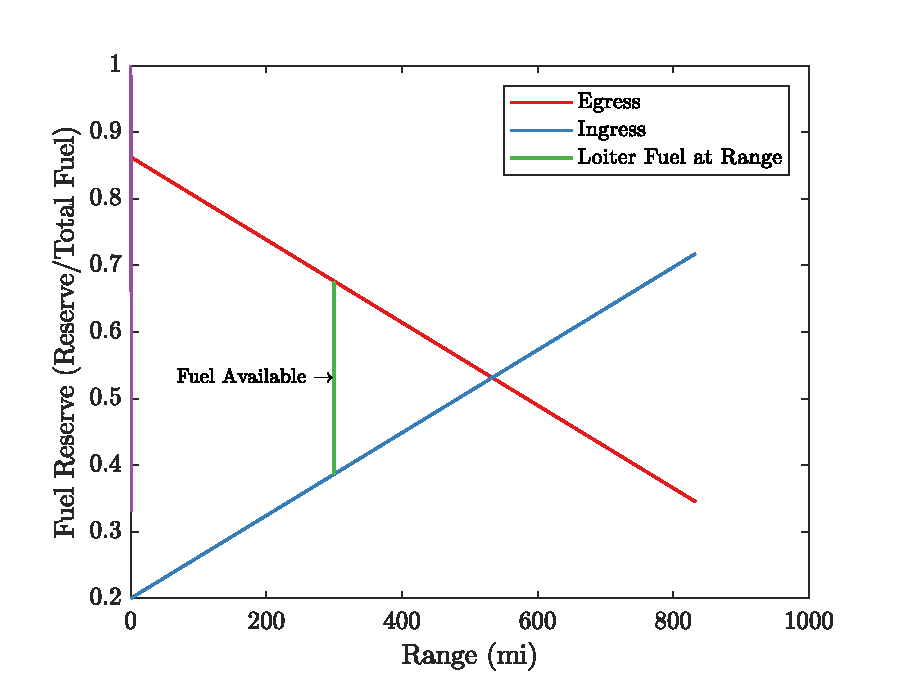
\includegraphics{Thesis/Method/ExampleFlightT37.eps}
    \caption{Example Flight Plan T-37}
    \label{fig:exT37}
\end{figure}
\subsection*{Non-linear Range Determination}
The non-linear equation for range is the equivalent formula presented in Eq. \ref{eq: NLRange}. The only additional parameter needed to solve for maximum range in this equation is the velocity which is assumed constant at the $C_L/C_D$. This is equivalent to finding the velocity at the maximum $\dfrac{C_L^{1/2}}{C_D}$. In the example case, since the drag polars at each mach number are unknown, a velocity of 0.5 mach at sea level will be used. Solving Eq. \ref{eq: NLRange} for fuel reserve where $W_F$ is the full weight and $W_D$ is the dry weight of the aircraft, the egress equation becomes
\begin{equation}
    f_e = \dfrac{\exp\left[\left(\dfrac{-R}{V}\right)\dfrac{(TSFC)}{C_L/C_D}\right]W_F-W_D}{W_F - W_D}.
    \label{eq: NLEgressEq}
\end{equation}
The equation for ingress is similarly derived as 
\begin{equation}
    f_{in} =\dfrac{\exp\left[\left(\dfrac{R}{V}\right)\dfrac{(TSFC)}{C_L/C_D}\right]W_F-W_D}{W_F - W_D}.
    \label{eq: NLIngressEq}
\end{equation}
In order for the equations to accurately represent fuel reserve, the given intercept must be determined for fuel burned during climb to cruise and take-off as well as the intercept for fuel reserve required.\par
The computations for the ingress intercept requires fewer computations than the egress intercept. To compute the ingress intercept, the fuel reserve percentage must be converted to fuel using the known weights of the aircraft. The parameter $f_r$ is the fuel reserve percentage and $p_f$ is the resulting percentage of reserve fuel.
\begin{equation*}
    p_f = (W_F - W_D)f_r
\end{equation*}
Then the minutes of reserve is converted to an aircraft weight by rearranging Eq. \ref{eq:maxendurance}. This becomes
\begin{equation*}
    f_t = \exp\left[\dfrac{t*(TSFC)}{(L/D)_{max}}\right]W_F-W_D
\end{equation*}
where $t$ is the endurance time in reserve for the aircraft and $f_t$ is the total fuel needed to meet this requirement. This must in turn be converted into a ratio of fuel to be reserved, $p_i$.
\begin{equation*}
    p_i = \dfrac{f_t + p_f}{W_F-W_D}.
\end{equation*}
The translation of the ingress equation is then calculated by solving for the vertical intercept in Eq. \ref{eq: NLIngressEq} where range is zero.
\begin{align*}
    t_{in}&= \textit{ingress translation} \\ &=-\left(\dfrac{C_L}{C_D}\right)V\ln\left[\dfrac{W_D+W_Fp_i- W_Dp_i}{W_F}\right]\dfrac{1}{(TSFC)}
\end{align*}
The new equation for ingress with the fuel reserve calculation becomes
\begin{equation}
    r_{in} = \textit{fuel \% remaining} =\dfrac{\exp\left[\left(\dfrac{R-t_{in}}{V}\right)\dfrac{(TSFC)}{C_L/C_D}\right]W_F-W_D}{W_F - W_D}.
    \label{eq: NLIngressFull}
\end{equation}
After calculating the percentage fuel remaining after climb to cruise, $p_e$, a similar approach to solving for the egress translation can be used as in the ingress intercept. The difference is solving for the translation using the known point of distance and fuel to cruise (in the form of $p_e$). Shown below, the translation for ingress is solved by rearranging Eq. \ref{eq: NLRange}. 
\begin{align*}
    t_e &= \textit{egress translation}\\
    &=-\ln\left[\dfrac{p_e(W_F-W_D)+W_D}{W_F}\right]\dfrac{V}{TSFC}\left(\dfrac{C_L}{C_D}\right)-R_{cruise}
\end{align*}
where $R_{cruise}$ is equal to the distance that the aircraft travels when climbing to cruise. The resulting equation for egress with the translation accounting for take-off and climb to cruise is 
\begin{equation}
    r_e = \textit{fuel \% remaining} = \dfrac{\exp\left[\left(\dfrac{-(R+t_e)}{V}\right)\dfrac{(TSFC)}{C_L/C_D}\right]W_F-W_D}{W_F - W_D}.
    \label{eq: NLEgressEqFull}
\end{equation}
The flight map run on the T-37 in Figure \ref{fig:NLFlightPlanT37} shows a similar result as the linear range equation, but the flight can be further defined by the use of a specific velocity, $V$, or $C_L/C_D$. This is useful when defining flight plans in a combat area where velocity or angle of attack is not necessarily for maximum range.
\begin{figure}[H]
    \centering
    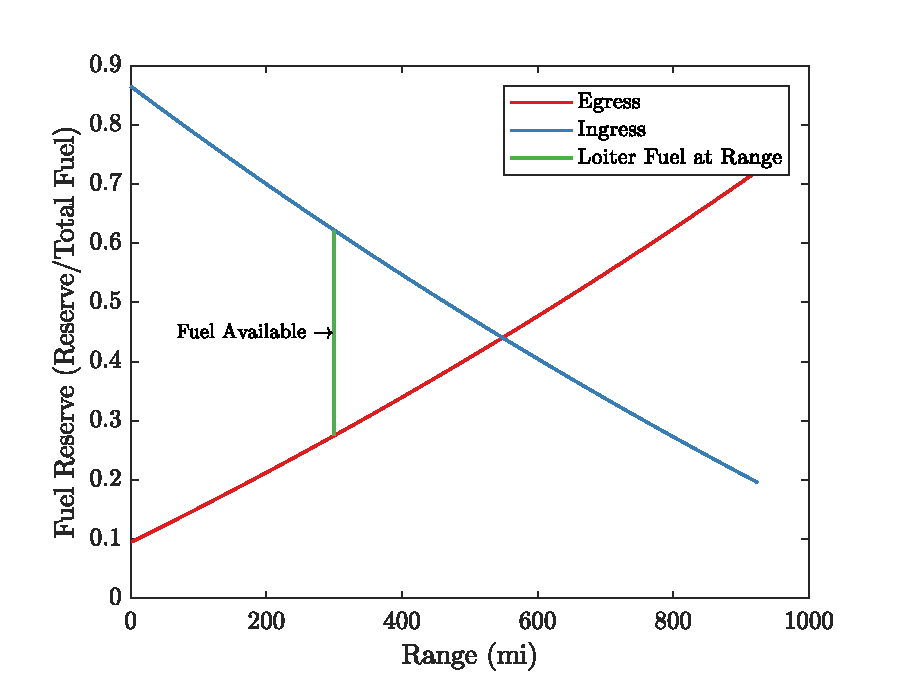
\includegraphics{Thesis/Method/NLFlightPlanT37.eps}
    \caption{Example Flight Plan for Nonlinear Br\'eguet Range Equation}
    \label{fig:NLFlightPlanT37}
\end{figure}
\par
%Remember to talk about 
% BELOW IS EXTRACTION
Parameters for the F-15C's $C_L\text{ and }C_D$ performance are referenced in Figure \ref{fig:machSpeedByGroup}. Each line in the graph represents a mach number which is formed by the value for each coefficient of lift ($C_L$) and the associated coefficient of drag ($C_D$). These are found from historical flying data for each specific aircraft. From the matrix of these values, the lift over drag and $C_L^{1/2}/C_D$ maximums can be found. Where $C_L^{1/2}/C_D$ is maximized, the respective mach number and $C_L/C_D$ can be pulled into the model as a parameter.\par
An example of F-15 drag polar outputs from the existing model are shown in Figure \ref{fig:machSpeedByGroup} for reference. Using the technique discussed above, the maximum values for $C_L/C_D$ and $C_L^{1/2}/C_D$ can be found from the matrix. An example of the matrix is shown in Section \ref{section:dragpolar}.

\begin{figure}[H]
    \centering
    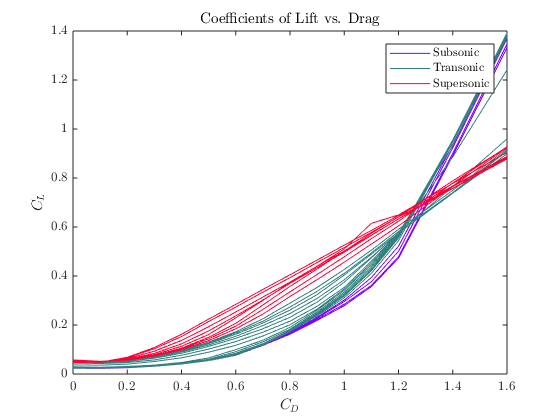
\includegraphics{Thesis/Method/MachSpeedByGroup.png}%
    \caption{Coefficients of lift versus drag for the F-15C.}%
    \label{fig:machSpeedByGroup}%
\end{figure}
\section{Loiter Time Determination}
Loiter time is determined based on Eq. \ref{endure}. Solving for the weight at the given range along the ingress and egress equations, the available loiter time can be determined over the target area. The endurance, $E_{available}$, can be caluclated using the following incorporation of the ingress and egress equation.

\begin{equation}
    E_{available} = \dfrac{1}{TSFC}\left(\dfrac{C_L}{C_D}\right)\ln\left(\dfrac{(r_e+ W_D)/W_F}{(r_{in}+W_D)/W_F}\right)
\end{equation}

This is used as a starting point for available minutes given that the aircraft has gone a certain range. The next step incorporates any combat time or climb from loiter or combat altitude. 

\section{Model Usage for Correction Factors}
\label{section:modelUsage}
The developed model adjusts for several parameters that are provided for comparing the NASIC model to the proposed model. These include given coefficients of lift, coefficients of drag, thrust specific fuel consumption at altitude, payload weights ($W_P$), external fuel tank weights ($W_{FT}$), total fuel weight ($W_{Fuel}$), internal fuel weight ($W_{int}$) take-off weight ($W_F$), combat fuel burn ($f_{com}$), and climb back to altitude after combat and/or loiter ($f_{climb}$). Dry weight, a corrected egress and ingress equation, and thrust specific fuel consumption at sea level can be determined from there. Additionally, an adjustment for including combat and the secondary climb to altitude must be determined for a true comparison.\par
Dry weight is found by using the take-off weight as a total weight and subtracting the total fuel weight such that $W_D = W_F - W_{Fuel}$. This is useful as the corrected ingress equation uses this as the final weight for range. The ingress equation must account for an external fuel tank and payload drop prior to combat.\par
The corrected ingress equation uses an additional derived parameter for full weight given that there are no external tanks or additional payload. In this way, the equations are corrected so that the egress equation uses an aircraft with the additional payload and external fuel tanks with the total fuel weight as its take-off weight and the dry weight as the final empty weight such that $W_{D_e} = W_{F_e}-W_{Fuel}$. The ingress equation uses the full weight of the aircraft given that there are no external fuel tanks, additional payloads, or any external fuel such that $W_{D_{in}} = W_F-W_{FT}-W_P - W_{Fuel}$ and $W_{F_{in}} = W_{D_{in}} + W_{int}$. \par
The two equations must also correct for the given flight plan, which includes a new $L/D$. $L/D$ is given at several weight steps for each aircraft by the NASIC output and the $L/D$ for the proposed model averages the weight steps that include any weight that the aircraft would be at during flight. For example, if the full weight of the aircraft is $40,000$ the $L/D$s at each weight step of $40,000$ or below would be averaged. The same is done for mach number and $TSFC$, but $TSFC$ must be adjusted for altitude.\par
Since $TSFC$ is brought into the model from an output at altitude, it must be adjusted to sea level in order for the proposed model to remain flexible at various altitudes. To do this, the temperature at altitude ($T_{alt}$) and the temperature at room temperature ($T$) are needed for Eq. \ref{eq:convTSFC}.
\begin{equation}
    TSFC = TSFC_{sl}\sqrt{T_{alt}/T}
    \label{eq:convTSFC}
\end{equation}
where temperature at altitude is found using the US Standard Atmosphere.
Solving for $TSFC$ at sea level will allow for conversions at each point  using Eq. \ref{eq:convTSFC} along the flight path when the altitude is changed for loiter or combat altitude. The final value for $TSFC$ will be divided by $3600$ to put the value in $TSFC/s$ instead of $TSFC/hr$. Similarly, mach number, $M$, will need to be converted to $ft/s$ using Eq. \ref{eq:convMach} given $T_{alt}$ and the gas constant ($R$), assuming the specific heat ratio of air for standard day conditions is $1.4$.
\begin{equation}
    V = 3.2808M\sqrt{1.4T_{alt}R}
    \label{eq:convMach}
\end{equation}
where $3.2808$ is the number of feet in a meter. This will also allow the model to remain agnostic to altitude given a mach number.\par
Converting the secondary climb to cruise altitude fuel burn and the combat fuel burn to a correction on the total available endurance is by converting the fuel burn to minutes lost. Using the dry weight of the ingress equation, minutes lost for secondary climb to cruise and combat can be found using Eq. \ref{eq:minlost} where $TSFC_{loiter}$ is the corrected $TSFC$ for loiter altitude.
\begin{equation}
\label{eq:minlost}
\begin{aligned}
    L_{com} &= \dfrac{1}{TSFC_{loiter}}\left(\dfrac{C_L}{C_D}\right)\ln\left(\dfrac{W_{D_{in}}+f_{com}}{W_{D_{in}}}\right)\\
    L_{climb} &=\dfrac{1}{TSFC_{loiter}}\left(\dfrac{C_L}{C_D}\right)\ln\left(\dfrac{W_{D_{in}}+f_{climb}}{W_{D_{in}}}\right).
\end{aligned}
\end{equation}
The final endurance value is then computed as $E = E_{avail}-L_{com}-L_{climb}$, where the full equation for determining $E_{avail}$ is shown in Eq. \ref{eq:EnduranceWithRange}. The algorithm has all the required parts for determining the Pareto front of endurance and range of the aircraft and a summary is shown in Algorithm \ref{Alg:R&E}. 
\begin{eqnarray}
\label{eq:EnduranceWithRange}
    E_{avail} & = &\dfrac{(C_L/C_D)}{TSFC_{loiter}}\left(TSFC_{alt}\dfrac{t_{in}-x}{V(C_L/C_D)}-\ln\left(W_{D_e}\right)\right) + \nonumber \\
    & &\dfrac{(C_L/C_D)}{TSFC_{loiter}}\ln\left(W_{D_{in}}-W_{D_e}+W_{F_e}\exp\left[-TSFC_{alt}\dfrac{t_e+x}{V(C_L/C_D)}\right]\right)
\end{eqnarray}
\begin{algorithm}[H]
\caption{Range and Endurance Algorithm}
\label{Alg:R&E}
\begin{algorithmic}
\Require{ac = Structure of Aircraft Parameters (ac.Parameter)}
\State $TSFC_{alt} = ac.TSFC\sqrt{T_{alt}/T}/3600$
\State $TSFC_{loiter} = ac.TSFC\sqrt{T_{loiter}/T}/3600$
\State $V = 3.2808*ac.M\sqrt{1.4T_{alt}R}$
\State $p_f = (ac.W_{F_{in}}-ac.W_{D_{in}})ac.f_r$
\State $f_t = \exp\left[\dfrac{ac.t*(TSFC_{alt})}{ac.(L/D)}\right]ac.W_{D_{in}}-ac.W_{D_{in}}$
\State $p_i = \dfrac{f_t + p_f}{ac.W_{F_{in}}-ac.W_{D_{in}}}$
\State $t_{in} = -ac.(L/D)V\ln\left[\dfrac{ac.W_{D_{in}}+(ac.W_{F_{in}}-ac.W_{D_{in}})p_i}{ac.W_{F_{in}}}\right]$
\State $t_e = -\ln\left[\dfrac{p_e(ac.W_{F_e}-ac.W_{D_e})+ac.W_{D_e}}{ac.W_{F_e}}\right]\dfrac{V}{TSFC_{alt}}ac.(L/D)-ac.R_{cruise}$
\State $L_{com} = \dfrac{1}{TSFC_{loiter}}ac.(L/D)\ln\left(\dfrac{ac.W_{D_{in}}+ac.f_{com}}{ac.W_{D_{in}}}\right)$
\State $L_{climb} = \dfrac{1}{TSFC_{loiter}}ac.(L/D)\ln\left(\dfrac{ac.W_{D_{in}}+ac.f_{climb}}{ac.W_{D_{in}}}\right)$
\For{x in k:n} 
\Comment{k,n is user-defined for distance between Pareto pts} 
    \State $r_{in}=\dfrac{\exp\left[\left(\dfrac{x-t_i}{V}\right)\dfrac{TSFC_{alt}}{ac.(L/D)}\right]ac.W_{D_{in}}-ac.W_{D_{in}}}{ac.W_{F_{in}} - W_{D_{in}}}$
    \State $r_e = \dfrac{\exp\left[\left(\dfrac{-(x+t_e)}{V}\right)\dfrac{(TSFC_{alt})}{ac.(L/D)}\right]ac.W_{F_e}-ac.W_{D_e}}{ac.W_{F_e} - ac.W_{D_e}}.$
    \State $E = \dfrac{1}{TSFC_{loiter}}ac.(L/D)\ln\left(\dfrac{(r_e+ ac.W_{D_e})/ac.W_{F_e}}{(r_{in}+ac.W_{D_{in}})/ac.W_{F_{in}}}\right) - L_{climb}-L_{com}$
    \State $E_{array} = E_{array}.append(E)$
    \State $R_{array} = R_{array}.append(x)$
\EndFor\\
\Return $T = [R_{array}, E_{array}]$ \Comment Return matrix for $T(row,:) = (range,endurance)$
\end{algorithmic}
\end{algorithm}
\section{Haversine Formula for Interest Locations}
\label{section:havMethod}
The Haversine formula calculates great-circle distance between two points on a sphere by latitude and longitude coordinates. The haversine formula of an angle is given as $\text{hav}(\theta) = \sin^2\left(\dfrac{\theta}{2}\right)$. The haversine formula is used to find distance, $d$, given the latitude and longitude of two points shown in Eq. \ref{eq:distHav}. 
\begin{equation}
\begin{aligned}
    a &= \sin^2\left(\dfrac{\phi_2-\phi_1}{2}\right)+\cos(\phi_1)\cos(\phi_2)\sin^2\left(\dfrac{\lambda_2-\lambda_1}{2}\right)
    \label{eq:distHav}\\
    d &= r*\text{atan2}(\sqrt{1-a},\sqrt{a})
\end{aligned}
\end{equation}
where $r$ is the radius of the sphere, $\phi_1,\phi_2$ are the latitudes of points 1 and 2, and $\lambda_1,\lambda_2$ are the longitudes of points 1 and 2. Given that the intersect can be calculated where endurance is equal to zero, the maximum range of the aircraft can be determined and then mapped. Figure \ref{fig:maxRadius} shows the maximum range of the F-15C from Salina, KS, in any direction. The perimeter of the range circle was found by solving for the longitude and latitude given the distance and the angle from the original location. \par
Using Eq. \ref{eq:distHav}, the distance from the initial point and various interest locations can be found given their latitude and longitude. The distance can then be evaluated as a range and the loiter time at that location can be found using the equations from the previous section. The result of finding the maximum endurance of an F-15C at the three locations of Dallas, TX, Oklahoma City, OK, and Denver, CO is shown in Figure \ref{fig:intPtsMap}. This method assumes that an aircraft will go out to the interest point and return to the initial location.
\begin{figure}
    \centering
    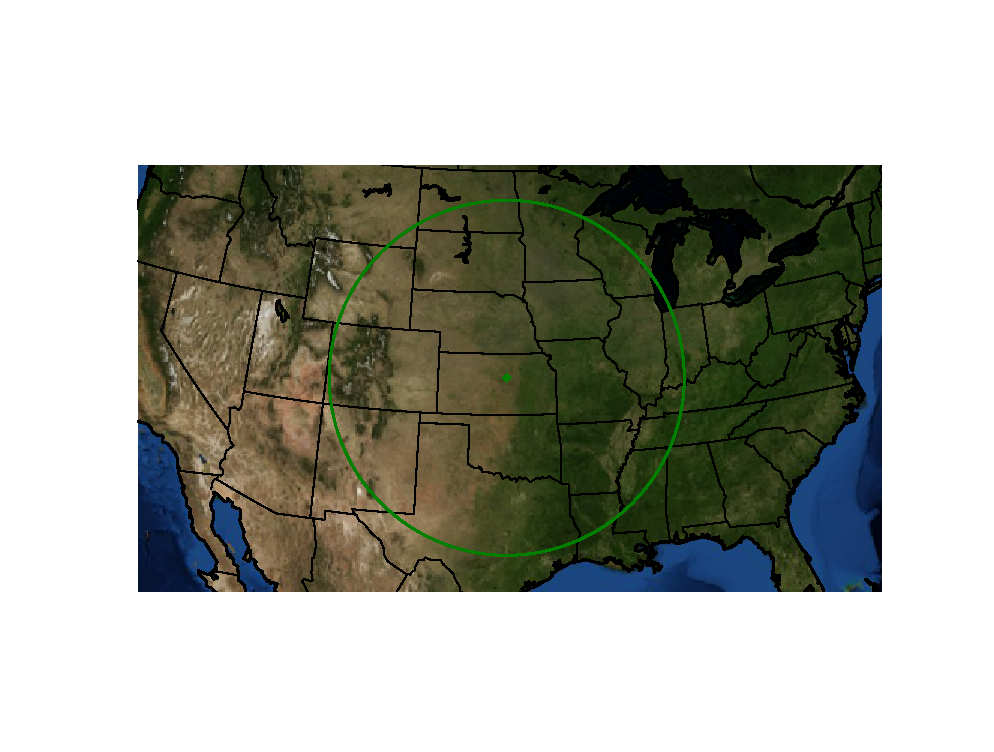
\includegraphics[width = 13cm]{Thesis/Method/RadiusEx.eps}
    \caption{Example maximum radius of F-15C mapped}
    \label{fig:maxRadius}
\end{figure}
\begin{figure}
    \centering
    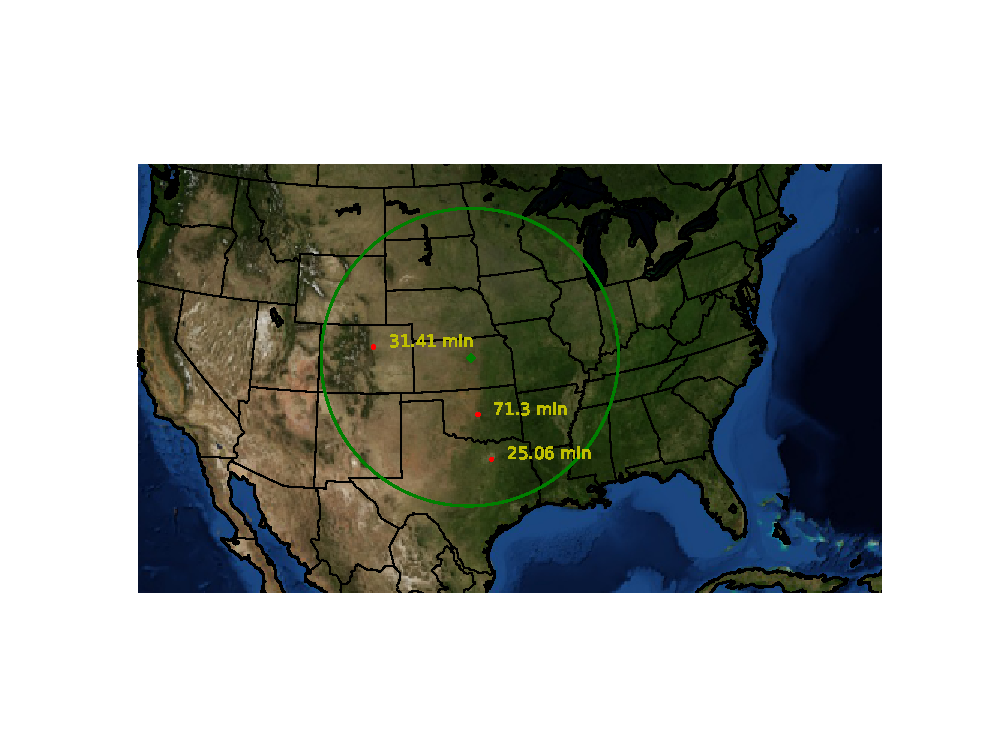
\includegraphics[width = 13cm]{Thesis/Method/IntPtsFigure.eps}
    \caption{Interest Points around Salina, KS}
    \label{fig:intPtsMap}
\end{figure}
